\section{Introduction}\label{sec:introduction}

\begin{figure}[tbp]
    \centering
    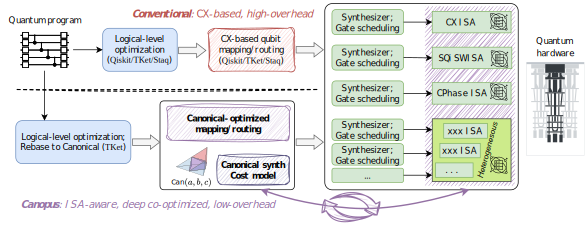
\includegraphics[width=\columnwidth,trim={0 0.5cm 0 0},clip]{figures/motivation.pdf}
    \caption{Compilation workflows by means of conventional approaches (top) and \canopus\ (bottom) targeting diverse quantum ISAs. \canopus\ integrates the synthesis cost model (monodromy polytopes within the Weyl chamber) by taking backend ISAs' properties into account. \canopus\ routing operates in the 2Q canonical representation while the specific synthesis is completed by the backend synthesizer.}
    %  \canopus\ exhibits a ISA-aware and deep co-optimized to achieve lower routing overhead.
    \label{fig:motivation}
\end{figure}


Quantum computing is a revolutionary computational paradigm leveraging quantum mechanics principles like superposition and entanglement of qubit states~\cite{nielsen2010quantum}. It has been rapidly growing in recent decades due to its potential speedups in task such as integer factorization~\cite{shor1994algorithms}, solving linear equations~\cite{harrow2009quantum}, and microscale system simulation~\cite{lloyd1996universal}. 


The holistic benchmarks of quantum computers such as quantum volume~\cite{cross2019validating} are predicated on concurrent advancements in both hardware and software. Recently numerous systematic techniques regarding compiler optimization and architectural support have been presented to push the limit of hardware performance. Quantum compiler plays a pivotal role in this process, translating high-level programs into executable single-qubit (1Q) and two-qubit (2Q) gates on realistic quantum hardware. This typically involves several critical stages: (1) compiling programs into basic quantum gates, (2) performing hardware-agnostic (logical-level) circuit optimization, (3) resolve backend topology constraints via qubit placement and routing, and (4) converting circuits to native gates for final optimization and scheduling. The primary goal of compiler optimization is to lower the 2Q gate count and circuit depth other than resolving backend constraints, as 2Q gates have significantly longer duration and higher error rate than 1Q gates. 

For mainstream quantum platforms like superconducting qubits~\cite{krantz2019quantum}, 2Q gates can only operate between the near-neighbor physical qubit pairs. Consequently, qubit placement and routing is crucial for resolving this connectivity constraint (e.g., Google's devices with 2D square topology~\cite{arute2019quantum}, IBM's devices with 2D heavy-hex topology~\cite{chamberland2020topological}), through dynamically remapping logical qubits to physical ones via inserting $ \SWAP $ gates acting on adjacent physical qubit pairs. Such induced routing overhead typically increase the gate count and circuit depth by a factor of 2x-4x relative to the pre-mapping circuits when using state-of-the-art (SOTA) scalable routing methods~\cite{li2019tackling,zulehner2018efficient,zhang2021time,liu2023tackling}. Therefore, mitigating this routing overhead remains a central and long-standing challenge in compiler optimization.


Most studies on qubit routing rely on a simplified routing model, where circuit cost is quantified by the $ \CX $-based gate count and circuit depth while each $ \SWAP $ gate is unrolled into three $ \CX $ gates according to the textbook pattern $ \SWAP_{q_0,q_1}=\CX_{q_0,q_1}\CX_{q_1,q_0}\CX_{q_0,q_1} $. However, this $ \CX $-centric view is misaligned with the physical reality of modern quantum systems. Although quantum algorithms are typically expressed in terms of $ \CX $ gates, the underlying hardware may not execute native $ \CX $-equivalent gates, nor does this gate/circuit cost quantification method accurately reflect the true operational cost. Indeed, beyond the native support for $ \CX $-equivalent gates (e.g., $ \CZ $~\cite{krantz2019quantum}, Cross-Resonance~\cite{rigetti2010fully}, Mølmer-Sørensen~\cite{bruzewicz2019trapped}), modern quantum hardwares increasingly feature diverse native 2Q basis gates in recent years. These alternative basis gates, or, the abstracted instruction set architectures (ISAs) in a narrow sense, could be more powerful than $ \CX $-equivalent gates in terms of synthesis capability and noise resilience, such as $ \SQiSW $~\cite{huang2023quantum}, fractional $ \iSWAP $-family or $ \CX $-family gates~\cite{mckinney2024mirage,qiskitXXDecomposer}, and heterogeneous/combinatorial basis gates~\cite{peterson2022optimal,mckinney2024mirage}. With such ISAs, $ \SWAP $ can be implemented with lower cost than three $ \CX $ gates or even be natively realized in high fidelity~\cite{yale2025realization,chen2025efficient,nguyen2024programmable}. Therefore, the gap between the simplified routing model and quantum ISAs' properties severely constrains the potential of compiler optimization, thereby limiting practical circuit execution performance. Conversely, the absence of systematic compiler optimization methods across these diverse (even complex, heterogeneous) ISAs has prevented the community from fully exploiting their power and exploring the rich software-hardware co-design space they enable.




% For example, the $ \SQiSW $ gate was proposed as a promising ISA by \citet{huang2023quantum}, as $ \SQiSW $ has the half duration of $ \iSWAP $ gate, thus with a $ 2\sqrt{2} $x speedup compared to the conventional $ \CZ $ gate scheme on flux-tunable superconducting transmons~\cite{krantz2019quantum}. Moreover, $ \SQiSW $ is of greater synthesis capability than $ CX $, as around 2.21 $ \SQiSW $ gates are sufficient to synthesis arbitrary (Haar-random) 2Q gates~\cite{huang2023quantum}, while the number is 3 for $ \CX $~\cite{shende2004minimal}. Recent experimental breakthroughs even demonstrate that arbitrary 2Q gates (including $ \SWAP $) can be natively implemented in high precision on both fixed-frequency~\cite{yale2025realization} and tunable-frequency~\cite{chen2025efficient} transmons. The hardware vendors, including IBM, Quantinuum, IonQ, etc., have newly supported fractional/partial entangling gates as their new-generation quantum ISAs~\cite{ibmFractionalGates,quantinuumArbitraryAngleGates,ionqPartialGates}. Particularly, the continuous $ \ZZ(\theta) $ gates (equivalent to $ \XX(\theta) $, $ \mathrm{ZX}(\theta) $, $ \mathrm{MS}(\theta) $ \ZY{MS gate???}, etc.) jointly adopted by them provides more synthesis capability, and the optimal 2Q synthesis functionality with a discrete fractional gate set $ \left\{\ZZ(\frac{\pi}{6}), \ZZ(\frac{\pi}{4}), \ZZ(\frac{\pi}{2})\right\} $ was already implemented in \qiskit~\cite{peterson2022optimal,qiskitXXDecomposer}. Although designing a good quantum ISA is an complicated task, those basis gates with greater synthesis capability, shorter gate duration, and higher calibration efficiency are potential to provide superior performance for real-world quantum applications. Typical instances are selected fractional $ \iSWAP $-family or $ \CX $-family gates and heterogeneous/combinatorial basis gates.





% .... 硬件发展。。。。 新型的ISA提出。。。
% 另一方面。。近年来量子硬件有了突破性进展。。。alternative ISA proposed 。。。 初步实现。。。单个basis gate有很好的特性(higher fidelity and powerful synthesis capability) 。。Compiler optimization上有很多挑战。。。但是如何利用、尤其如何统一地抵用他们、还没有系统化的探索。。。有一个unified利用方式以及以及如何评估不同ISA的实际性能是至关重要的

% 为了解决这些挑战,我们提出了一种framework。。。借助形式化的描述,。。。是的这一目标成为可能,验证了advanced ISA实际上带来的效果提升好过CNOT,而且进行了cross-ISA, program features, hardware topology的co-exploration


%  of diverse, complex or heterogeneous ISAs.

In our work, we propose a unified qubit mapping/routing framework \canopus\ (\fullNameOfCanopus) tailored to diverse quantum ISAs. Unlike conventional $ \CX $-based routing approaches, \canopus\ is fundamentally ISA-aware. As illustrated in \Cref{fig:motivation}, it incorporates the properties of the target ISA into a canonical cost model to perform deep co-optimization of routing and synthesis. By means of the formal, canonical representation of 2Q gates, \canopus\ fully exploit the synthesis capabilities of the given ISA. This approach demonstrates that advanced ISAs can achieve significantly lower routing overheads than conventional models suggest.


To perform unified qubit routing, \canopus\ leverages key insights: \ding{172} Considering the subsequent synthesis overhead with native basis gates into the qubit routing stage could unlock significant optimization opportunities. For instance, a $ \SWAP $ inserted after a 2Q block with the same qubit pair acted on could lead to a better synthesis result when rebased to the backend ISA. \ding{173} Expanding the quantum ISA is crucial to boost the performance of real-world quantum applications. For example, the fractional $ \ZZ(\theta) $ gate set that is widely adopted by hardware vendors (e.g.,IBM~\cite{ibmFractionalGates}, Quantinuum~\cite{quantinuumArbitraryAngleGates}, IonQ~\cite{ionqPartialGates}) apparently enables more efficient execution for chemistry simulation kernels within which many 2-local Pauli rotations are involved. The combination of $ \CX $ and $ \iSWAP $ gates have been demonstrated to benefit stabilizer circuits to protect error-corrected qubit information. \ding{174} Canonical representation of 2Q gates~\cite{zhang2003geometric} and the monodromy polytope theory~\cite{peterson2020fixed} provides a formal, universal, and quantitative description of the 2Q synthesis cost for generic quantum ISAs. This formalism enables the possibility of unified compiler optimization.\quad With these insights in mind, \canopus\ performs intelligent $ \SWAP $ insertion during qubit routing to globally minimize post-mapping circuit cost (in terms of both count and depth) given any quantum ISA, thus performing deep routing-synthesis co-optimization and resulting in significantly lower routing overhead. Importantly, although \canopus\ is ISA-aware, it always operate on the canonical-form circuits, and the gate/circuit cost quantification via monodromy polytopes is irrespective to specific ISA rebase implementation. Thus \canopus\ offers an LLVM-style optimization. 


% Our framework can be extended to integrate more fine-grain hardware information such as qubit-specific basis gate fidelities.

Experimental results demonstrate that \canopus\ provides 30\%-40\% reduction of routing overhead compared to other SOTA methods across representative quantum ISAs, including the conventional \CXISA\ ISA. This coherent cross-ISA comparison also reveals some consistent or program-specific or topology-specific guidelines for hardware-software co-design. Furthermore, our case studies of the real-machine experiment for QFT kernel execution on 1D chain topology and the end-to-end QEC circuit simulation demonstrates the practical superiority of \canopus\ in both NISQ and fault-tolerant applications. Source code and data are available via the \canopusGitHub~\cite{canopusGitHub}.

% \note{Our work addresses the \dquote{Babel Tower dilemma} in quantum compilation by establishing a canonical language for diverse two-qubit gates, enabling unified optimization across heterogeneous quantum ISAs.} 

Our work makes the following key contributions:
\begin{itemize}
  \item We propose \canopus, the first unified qubit routing framework applicable to diverse quantum ISAs. Unlike conventional methods fixed on a $\CX$-based routing paradigm, \canopus is fundamentally ISA-aware and operates on the canonical-form circuits, able to exploit the unique capabilities of any given quantum ISA.
  % designed to operate across diverse quantum ISAs. Unlike conventional methods fixed on a $\CX$-based model, \canopus is fundamentally ISA-aware, enabling it to exploit the unique synthesis capabilities of any given hardware.
  \item We utilize the canonical 2Q gate representation and the monodrome polytope theory to quantify costs of 2Q gates and the overall circuit. This formal approach accurately guides synthesis-routing co-optimization and cross-ISA evaluation. 
  \item We formalize the analysis of commutation relations between arbitrary 2Q canonical gates that share one qubit. This offers a generalized commutativity-based optimization mechanism, moving beyond those tailored only for $\CX$ gates~\cite{liu2022not}.
  % \item We propose sophisticated heuristic algorithms and data structures that balance the gate count related circuit cost and circuit depth related circuit cost.
  \item We conduct comprehensive experiments across a wide range of real-world benchmarks, hardware topologies, and representative ISAs, showing that \canopus\ consistently reduces routing overhead by 30\%-40\% compared to SOTA methods. Our results also yield coherent guidelines for the co-design of quantum programs, ISAs, and hardware topologies. 
  \item We validate that theoretically expressive ISAs has superior performance than the conventional \CXISA\ ISA, not as what we traditionally believe according to prior works~\cite{kalloor2024quantum}. Furthermore, \canopus\ confirms that the routing-synthesis co-optimization is a unified, highly-effective compiler optimization paradigm to utilized advanced quantum ISAs.
  \item Our case studies, including the real-machine QFT kernel execution and the end-to-end QEC circuit simulation, unequivocally showcase \canopus' superiority in both near-term and fault-tolerant applications. For example, on the task of mapping QFT on 1D chain topology, \canopus\ finds the provably optimal routing scheme, surpassing the results previously reported as optimal in prior work~\cite{zhang2021time}; and experiments on IBM's QPUs suggests that \canopus\ leads to an average \note{5x} error reduction compared to \qiskit.
\end{itemize}







% Our main contributions are summarized as follows: \ZY{Technical contribution}
% \begin{itemize}
%     \item We introduce \canopus\, a unified qubit routing framework based on the canonical 2Q gate representation 
%     \item Canonical ... gate synthesis ... ... synthesis cost model ... monodromy polytopes
%     \item We systematically ... unified qubit routing framework ... utilizing advanced ISAs ... demonstrate the practical superiority of advanced quantum ISAs ...  addresses the \dquote{Babel Tower dilemma} 
%     \item Heuristic cost function ... 
%     \item In our findings, the  commutative optimization by means of canonical representation, ... canonical gate commutation relations in our findings
%     \item Evaluation cross-ISA, co-exploration ...
%     \item Case studies (QFT, QEC) .... real quantum computer experiment ... FTQC
% \end{itemize}




% does not introduce higher computational complexity
% is compatible with existing routing techniques


% Implementation of \canopus\ is based on the \qiskit\ SDK and the newly introduced calculation mechanism  

% Implementation of \canopus\ is based on the 





% compiler optimization dedicated to $ \SQiSW $ basis gate~\cite{tang2024quantum,mckinney2024mirage} demonstrates its practical usage other than 2Q gate ...  is ...  the combination of $ \CX $ and $ \iSWAP $ gates

% circuit synthesis theory .... 
% in real-world applications



% orthodox


% - 高屋建瓴介绍 ... 证明advanced ISA的结果更好
% - key insight / key methodology: conventional routing paradigm is insufficient ... synthesis-routing co-optimization is important: canonical and monodromy poloytopes ... formal description is a unified, generalized quantification ..%. (应该说是technical insight)
% - 结果
% Although there is attempts~\cite{liu2022not,mckinney2024mirage} under the consensus that not all $ \SWAP $ insertions cost the same, they are either limited to $ \CX $-based 




% \canopus\ (\fullNameOfCanopus) is a qubit mapping and routing framework that is tailored to advanced quantum ISAs, such as $\Can$~\cite{chen2024one} and $\SQiSW$~\cite{huang2023quantum}, which are adaptive to versatile hardware architectures. \canopus\ is designed to optimize the placement of qubits and the routing of quantum gates, taking into account the specific requirements of these advanced ISAs.



